\chapter{Motivation: the $2^{B}$ trajectory space}
\label{ch:motivation}

Before we invest in any search algorithm, two questions need answers. Does the space of binary masks contain visually different outcomes, or do they all collapse to the same edit? Does the all-target mask $M=\mathbf{1}$ already solve the editing problem, making the search pointless? This chapter answers both by running exhaustive search on two Stable Diffusion~v1.5 editing tasks and analysing the $2^{20}\approx 10^6$ outputs.

\section{Setup}

\paragraph{Cat $\to$ Dog.} Source: ``tabby kitten walking confidently across a stone pavement.'' Target: ``tabby dog walking confidently across a stone pavement.'' Species swap over an urban background.

\paragraph{Horse $\to$ Robot Horse.} Source: ``a horse on the grass.'' Target: ``a robot horse on the grass.'' Appearance swap (organic to mechanical) over a natural background.

\begin{figure}[H]
    \centering
    \begin{subfigure}[b]{0.4\textwidth}
        \centering
        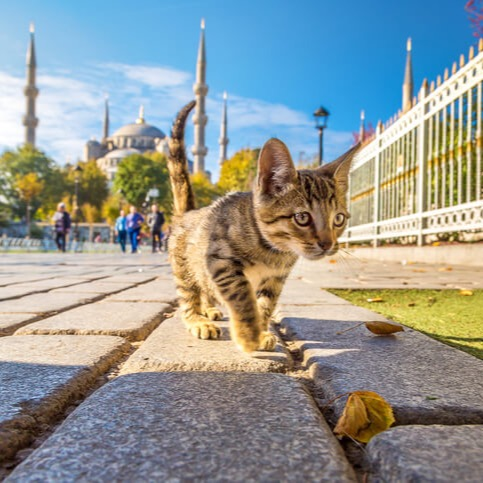
\includegraphics[width=\textwidth]{images/source_catdog.jpg}
        \caption{Cat $\to$ Dog source image.}
    \end{subfigure}
    \hspace{0.04\textwidth}
    \begin{subfigure}[b]{0.4\textwidth}
        \centering
        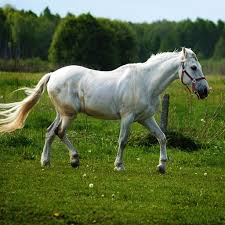
\includegraphics[width=\textwidth]{images/source_horse.jpg}
        \caption{Horse $\to$ Robot Horse source image.}
    \end{subfigure}
    \caption{Source images for both motivational editing tasks.}
    \label{fig::source_images}
\end{figure}

One source image per task. For each task we enumerate every $M\in\{0,1\}^{20}$ and generate the image. Table~\ref{tab::hyperparams} lists the pipeline settings.

\begin{table}[H]
    \centering
    \caption{Exhaustive-search setup.}
    \begin{tabular}{ll}
    \toprule
    Base model & Stable Diffusion v1.5 \\
    Scheduler & DDIM, scaled linear $\beta$ \\
    Steps / Mask bits & $T=40$, $B=20$, $R=2$ \\
    Guidance / Resolution & $s=7.5$, $512\times512$ \\
    Precision & FP32 inversion, FP16 sampling \\
    Hardware & $8\times$ A100 80GB \\
    Features & DINOv2 ViT-S/14, CLIP ViT-B/32 \\
    Segmentation & CLIPSeg-RD64 + SAM ViT-B \\
    \bottomrule
    \end{tabular}
    \label{tab::hyperparams}
\end{table}

Reward follows Equation~\ref{eq::objective_exh}: the geometric mean of min-max normalised background SSIM and foreground CLIP score.

\section{The trajectory space has structure}

HDBSCAN on UMAP-projected DINOv2 features of the $\sim\!1$M cat$\to$dog outputs returns 52 clusters; the horse task returns 13 (Figure~\ref{fig::cluster_maps}). Figure~\ref{fig::cluster_grids} shows five sample images per cluster for the six largest clusters of each task.

\begin{figure}[H]
    \centering
    \begin{subfigure}[t]{0.48\textwidth}
        \centering
        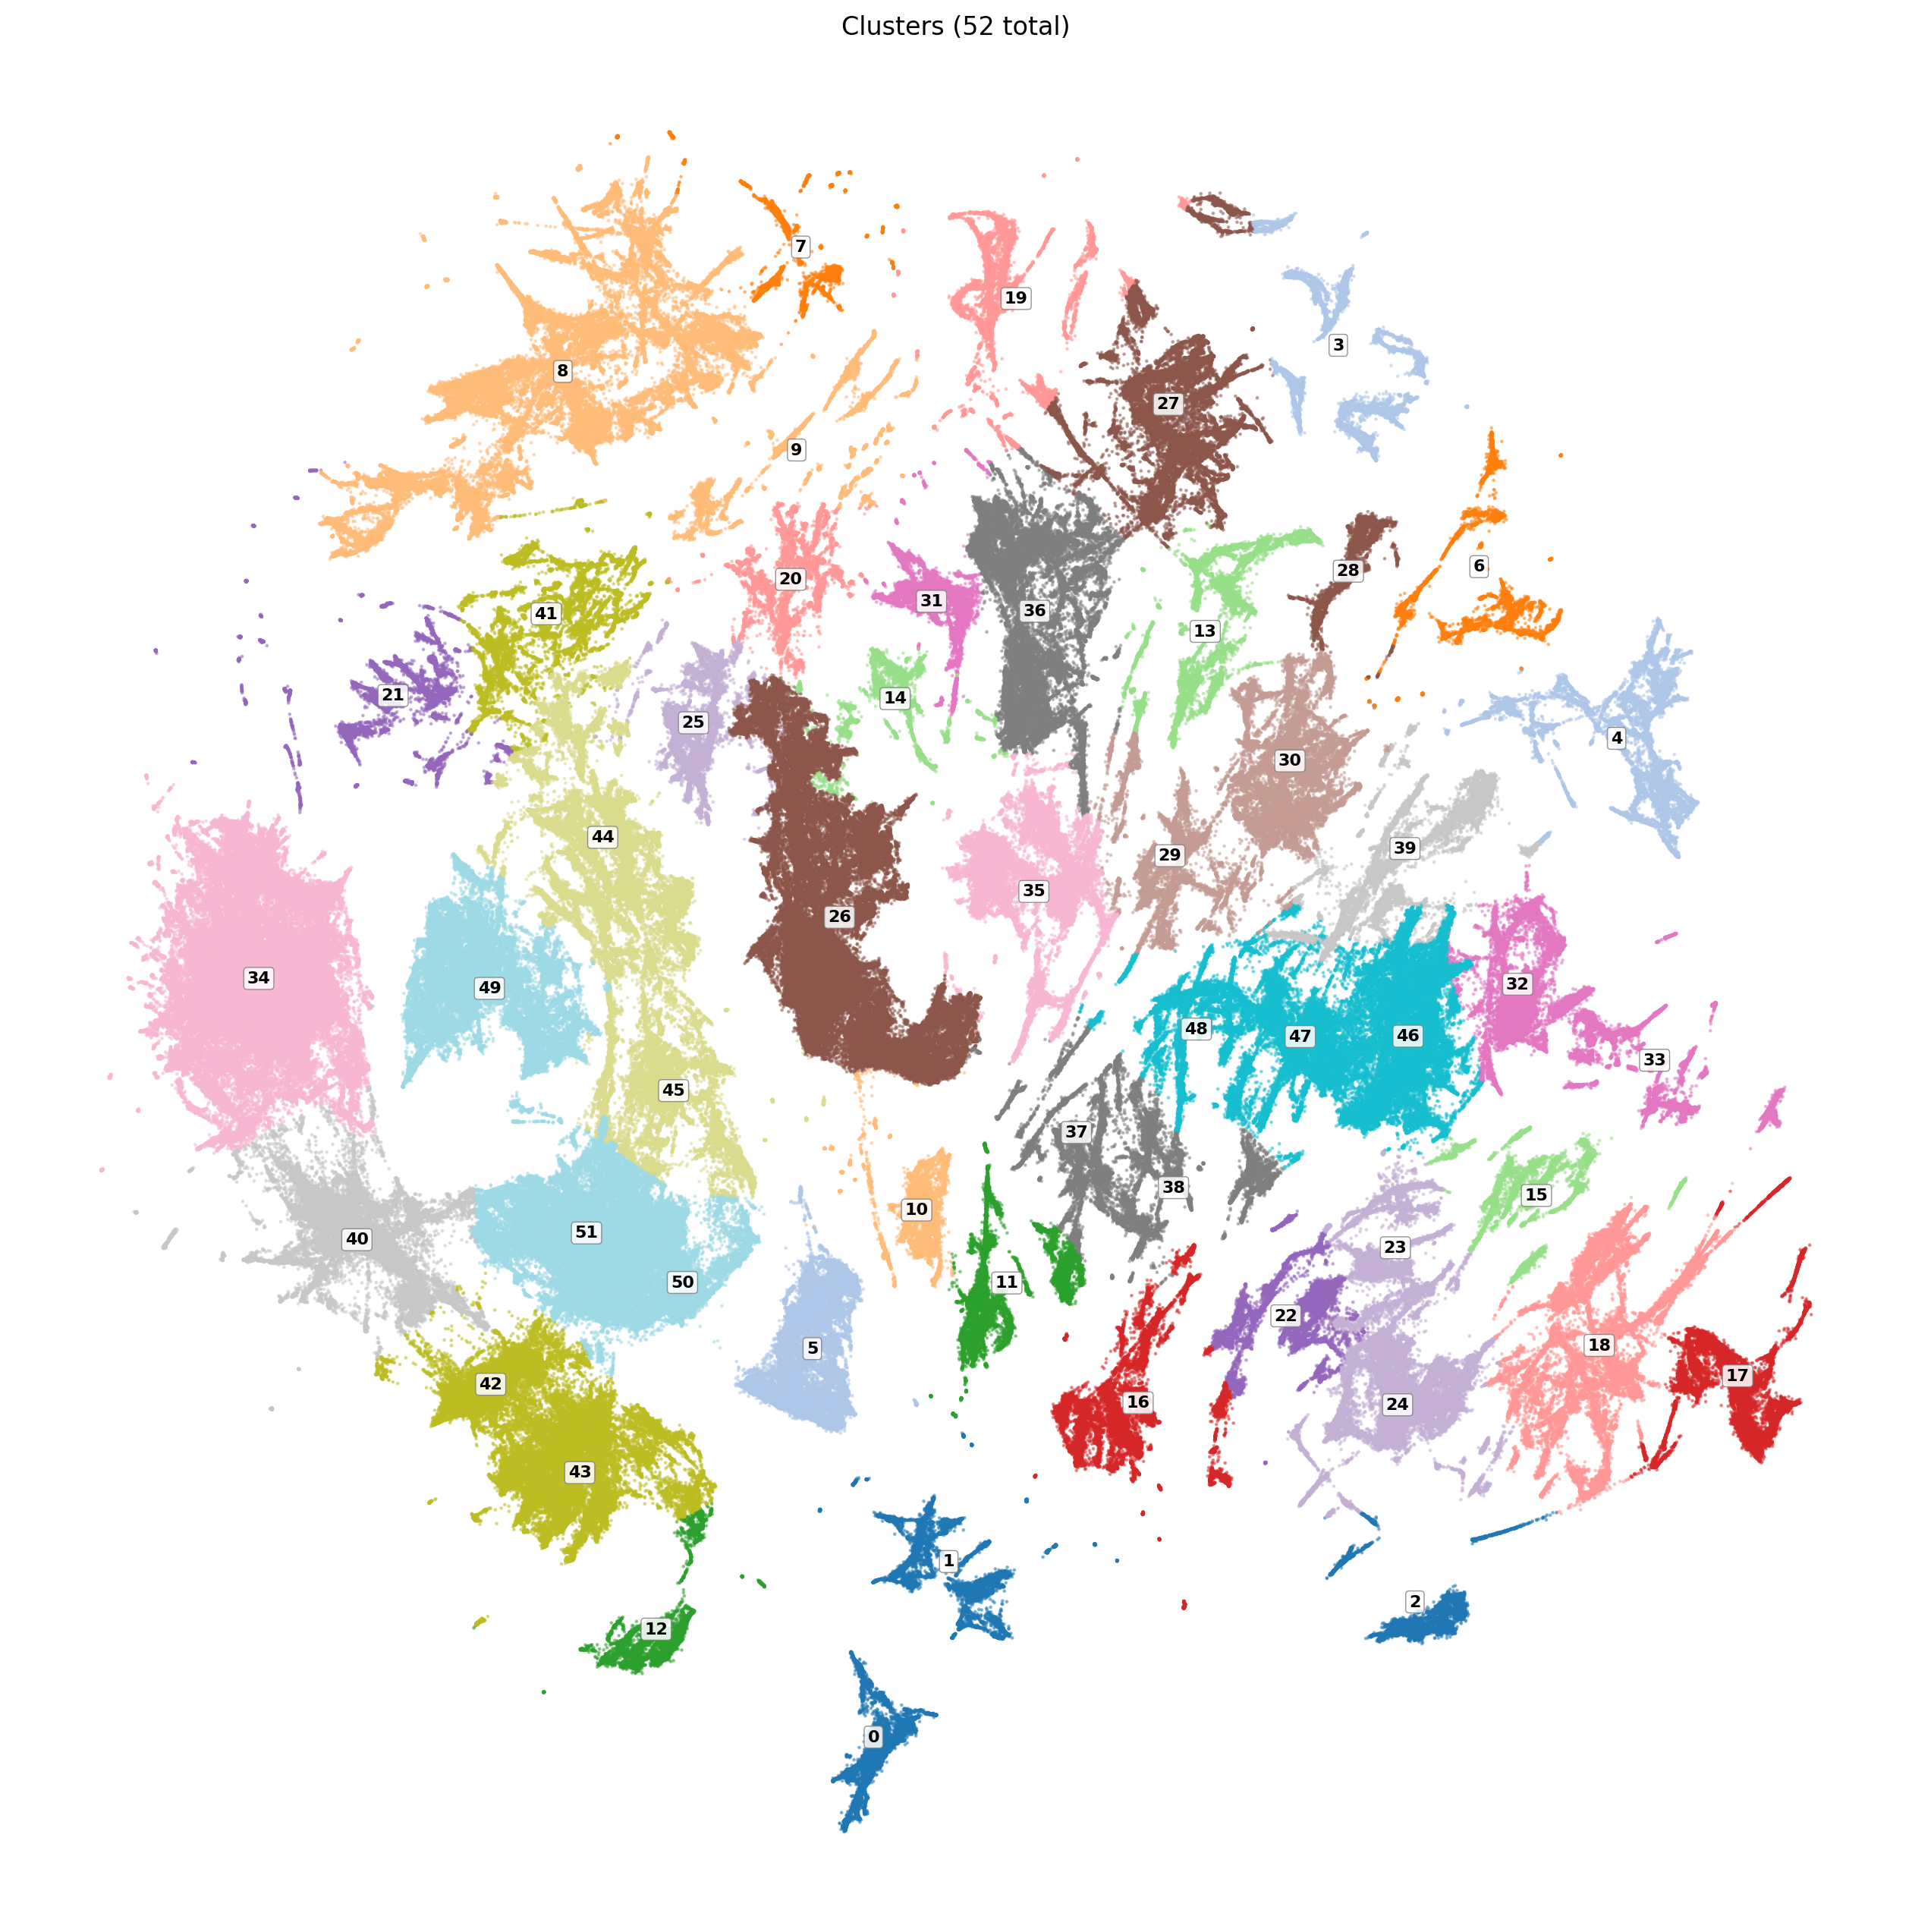
\includegraphics[width=\textwidth]{images/catdog_map_clusters.png}
        \caption{Cat$\to$dog, 52 clusters.}
        \label{fig::catdog_clusters}
    \end{subfigure}
    \hspace{0.02\textwidth}
    \begin{subfigure}[t]{0.48\textwidth}
        \centering
        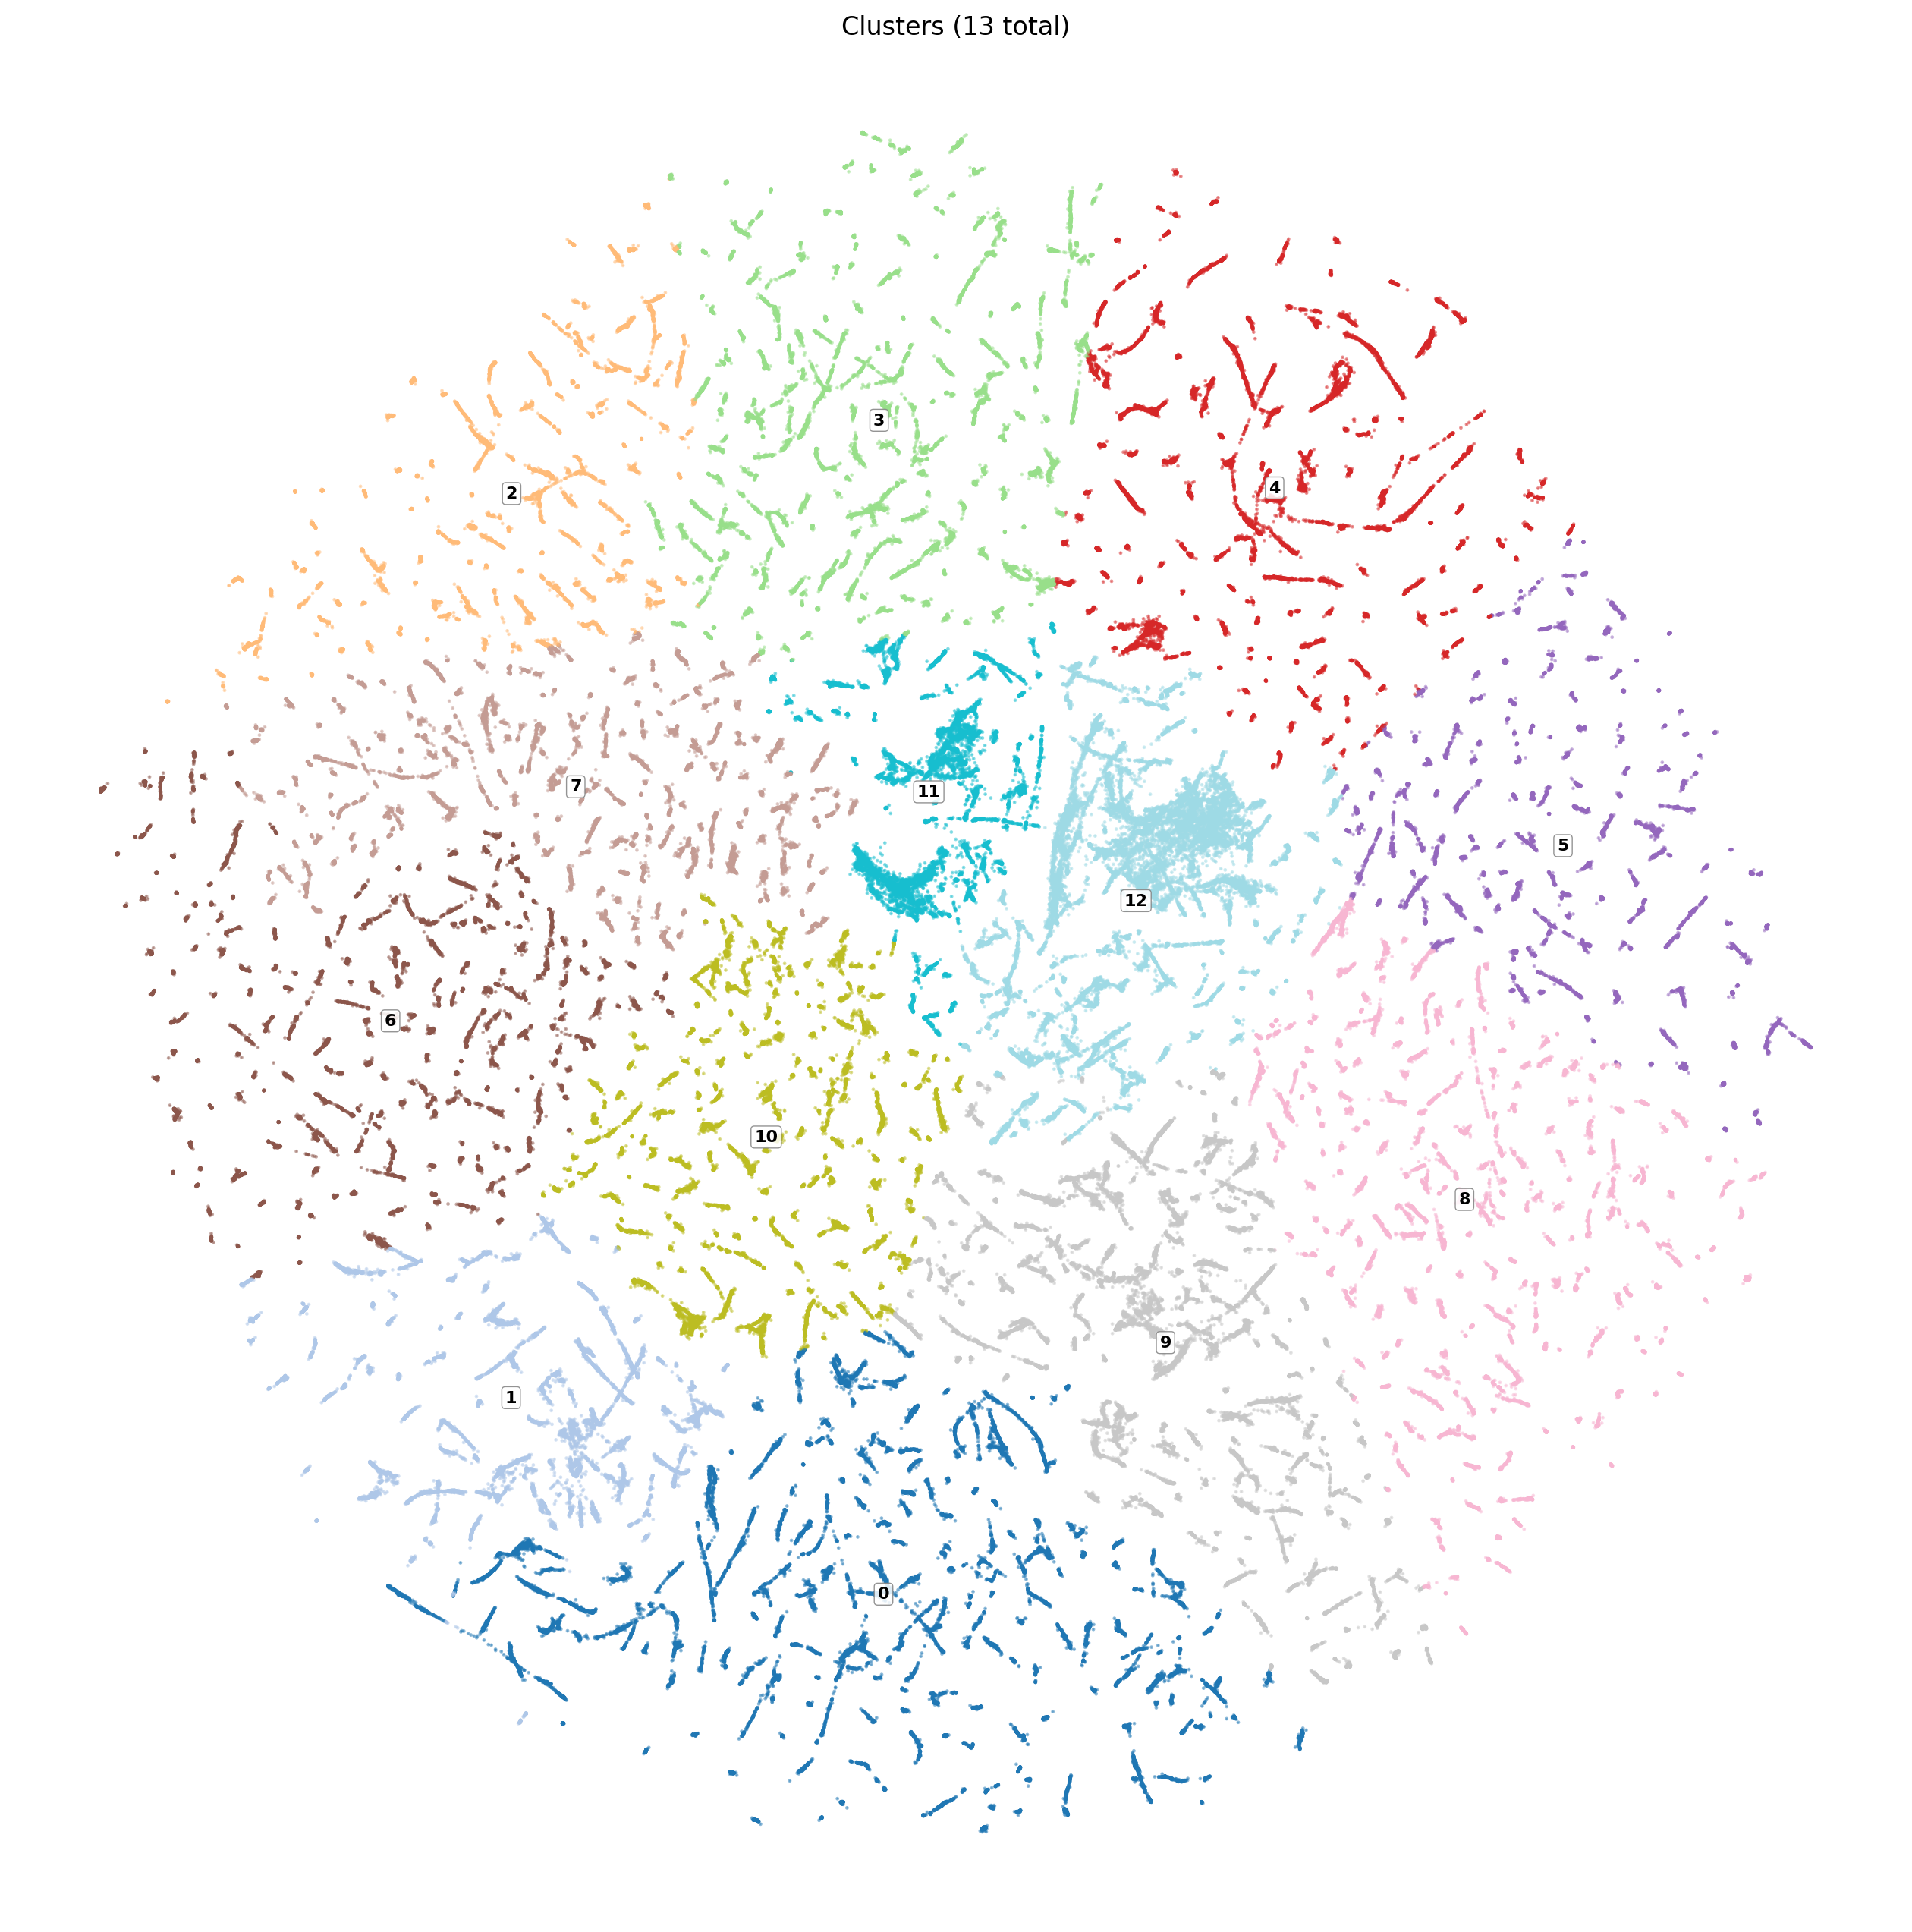
\includegraphics[width=\textwidth]{images/horse_map_clusters.png}
        \caption{Horse$\to$robot horse, 13 clusters.}
        \label{fig::horse_clusters}
    \end{subfigure}
    \caption{UMAP projections of the $\sim\!10^6$ outputs per task, coloured by HDBSCAN cluster.}
    \label{fig::cluster_maps}
\end{figure}

\begin{figure}[H]
    \centering
    \begin{subfigure}[t]{0.48\textwidth}
        \centering
        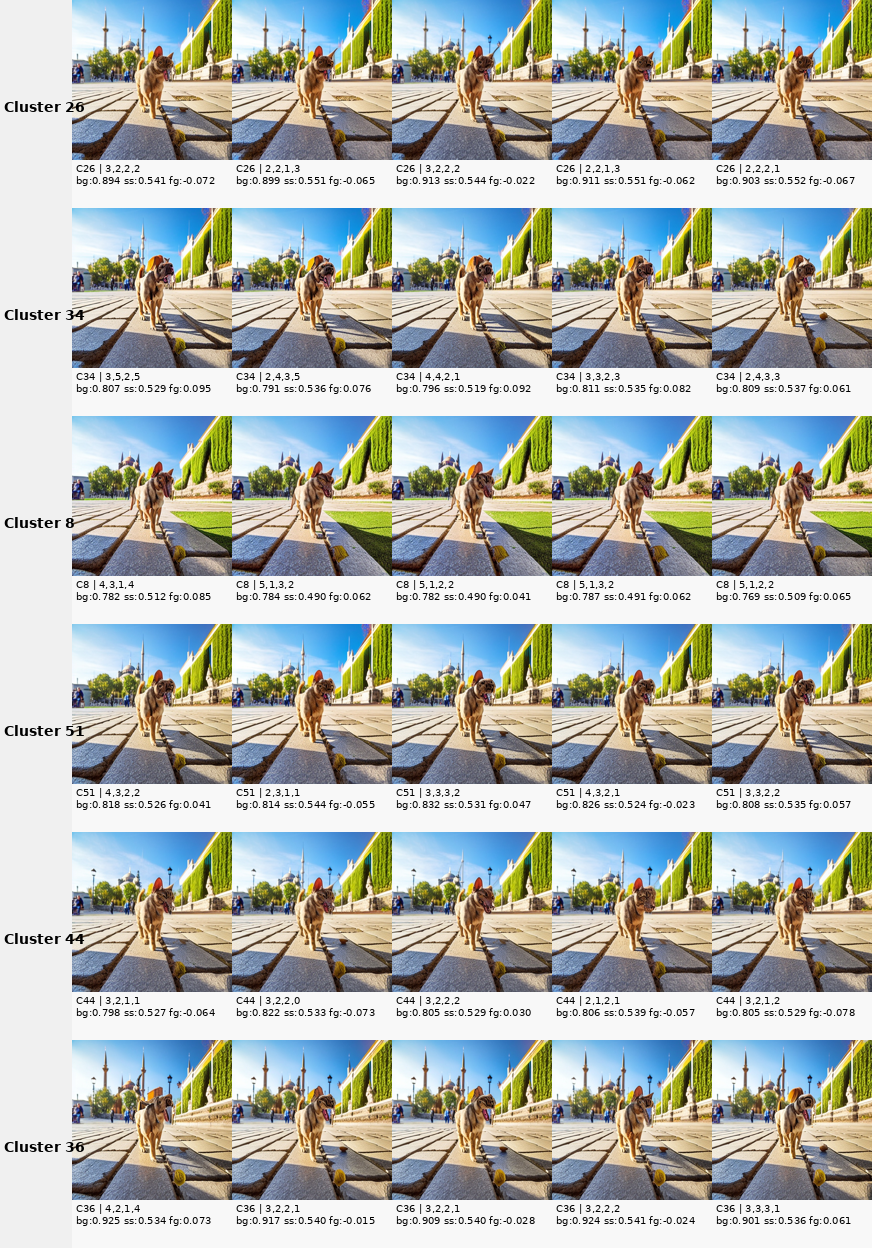
\includegraphics[width=\textwidth]{images/catdog_grid_top6_x5.png}
        \caption{Cat$\to$dog.}
        \label{fig::catdog_grid_clusters}
    \end{subfigure}
    \hspace{0.02\textwidth}
    \begin{subfigure}[t]{0.48\textwidth}
        \centering
        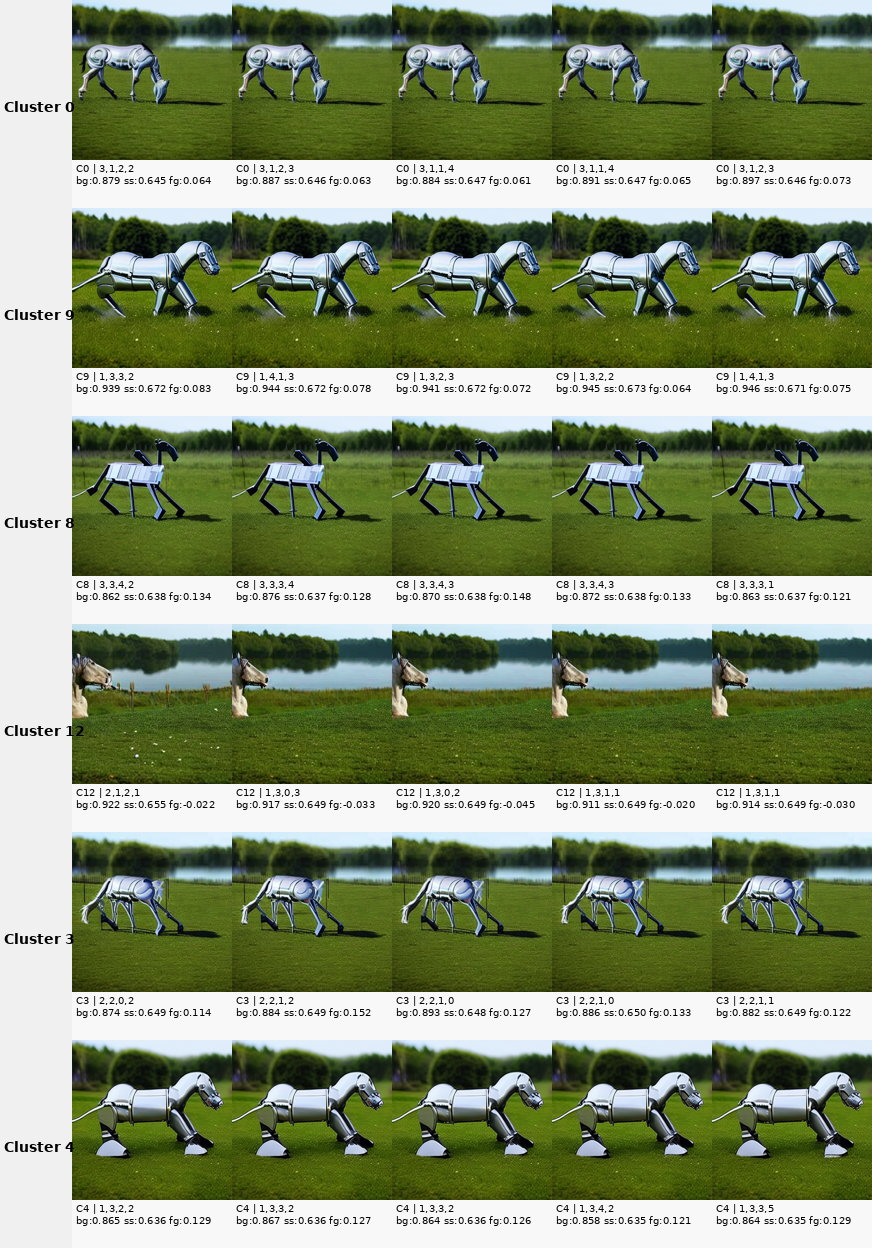
\includegraphics[width=\textwidth]{images/horse_grid_top6_x5.png}
        \caption{Horse$\to$robot horse.}
        \label{fig::horse_grid_clusters}
    \end{subfigure}
    \caption{Six largest clusters per task, 5 representative images per cluster (top to bottom). Annotations show cluster ID, quadrant activation pattern, and per-image metrics.}
    \label{fig::cluster_grids}
\end{figure}

Cat$\to$dog produces four times more clusters than horse$\to$robot horse. The cat$\to$dog edit changes species, so shape, fur, posture, and proportions all move; the horse edit keeps quadruped anatomy and changes surface appearance only. The trajectory space ranges from unchanged source images through intermediate morphs to fully-edited targets; cluster count tracks how much visual change the prompt demands.

The UMAP metric maps (Figure~\ref{fig::metric_maps}) show which regions score well on which sub-reward. Background preservation and foreground editability light up different UMAP regions. The combined score peaks in a narrow Pareto band between the two. Nearby masks give similar scores, so the reward surface is locally smooth.

\begin{figure}[H]
    \centering
    \begin{subfigure}[t]{0.48\textwidth}
        \centering
        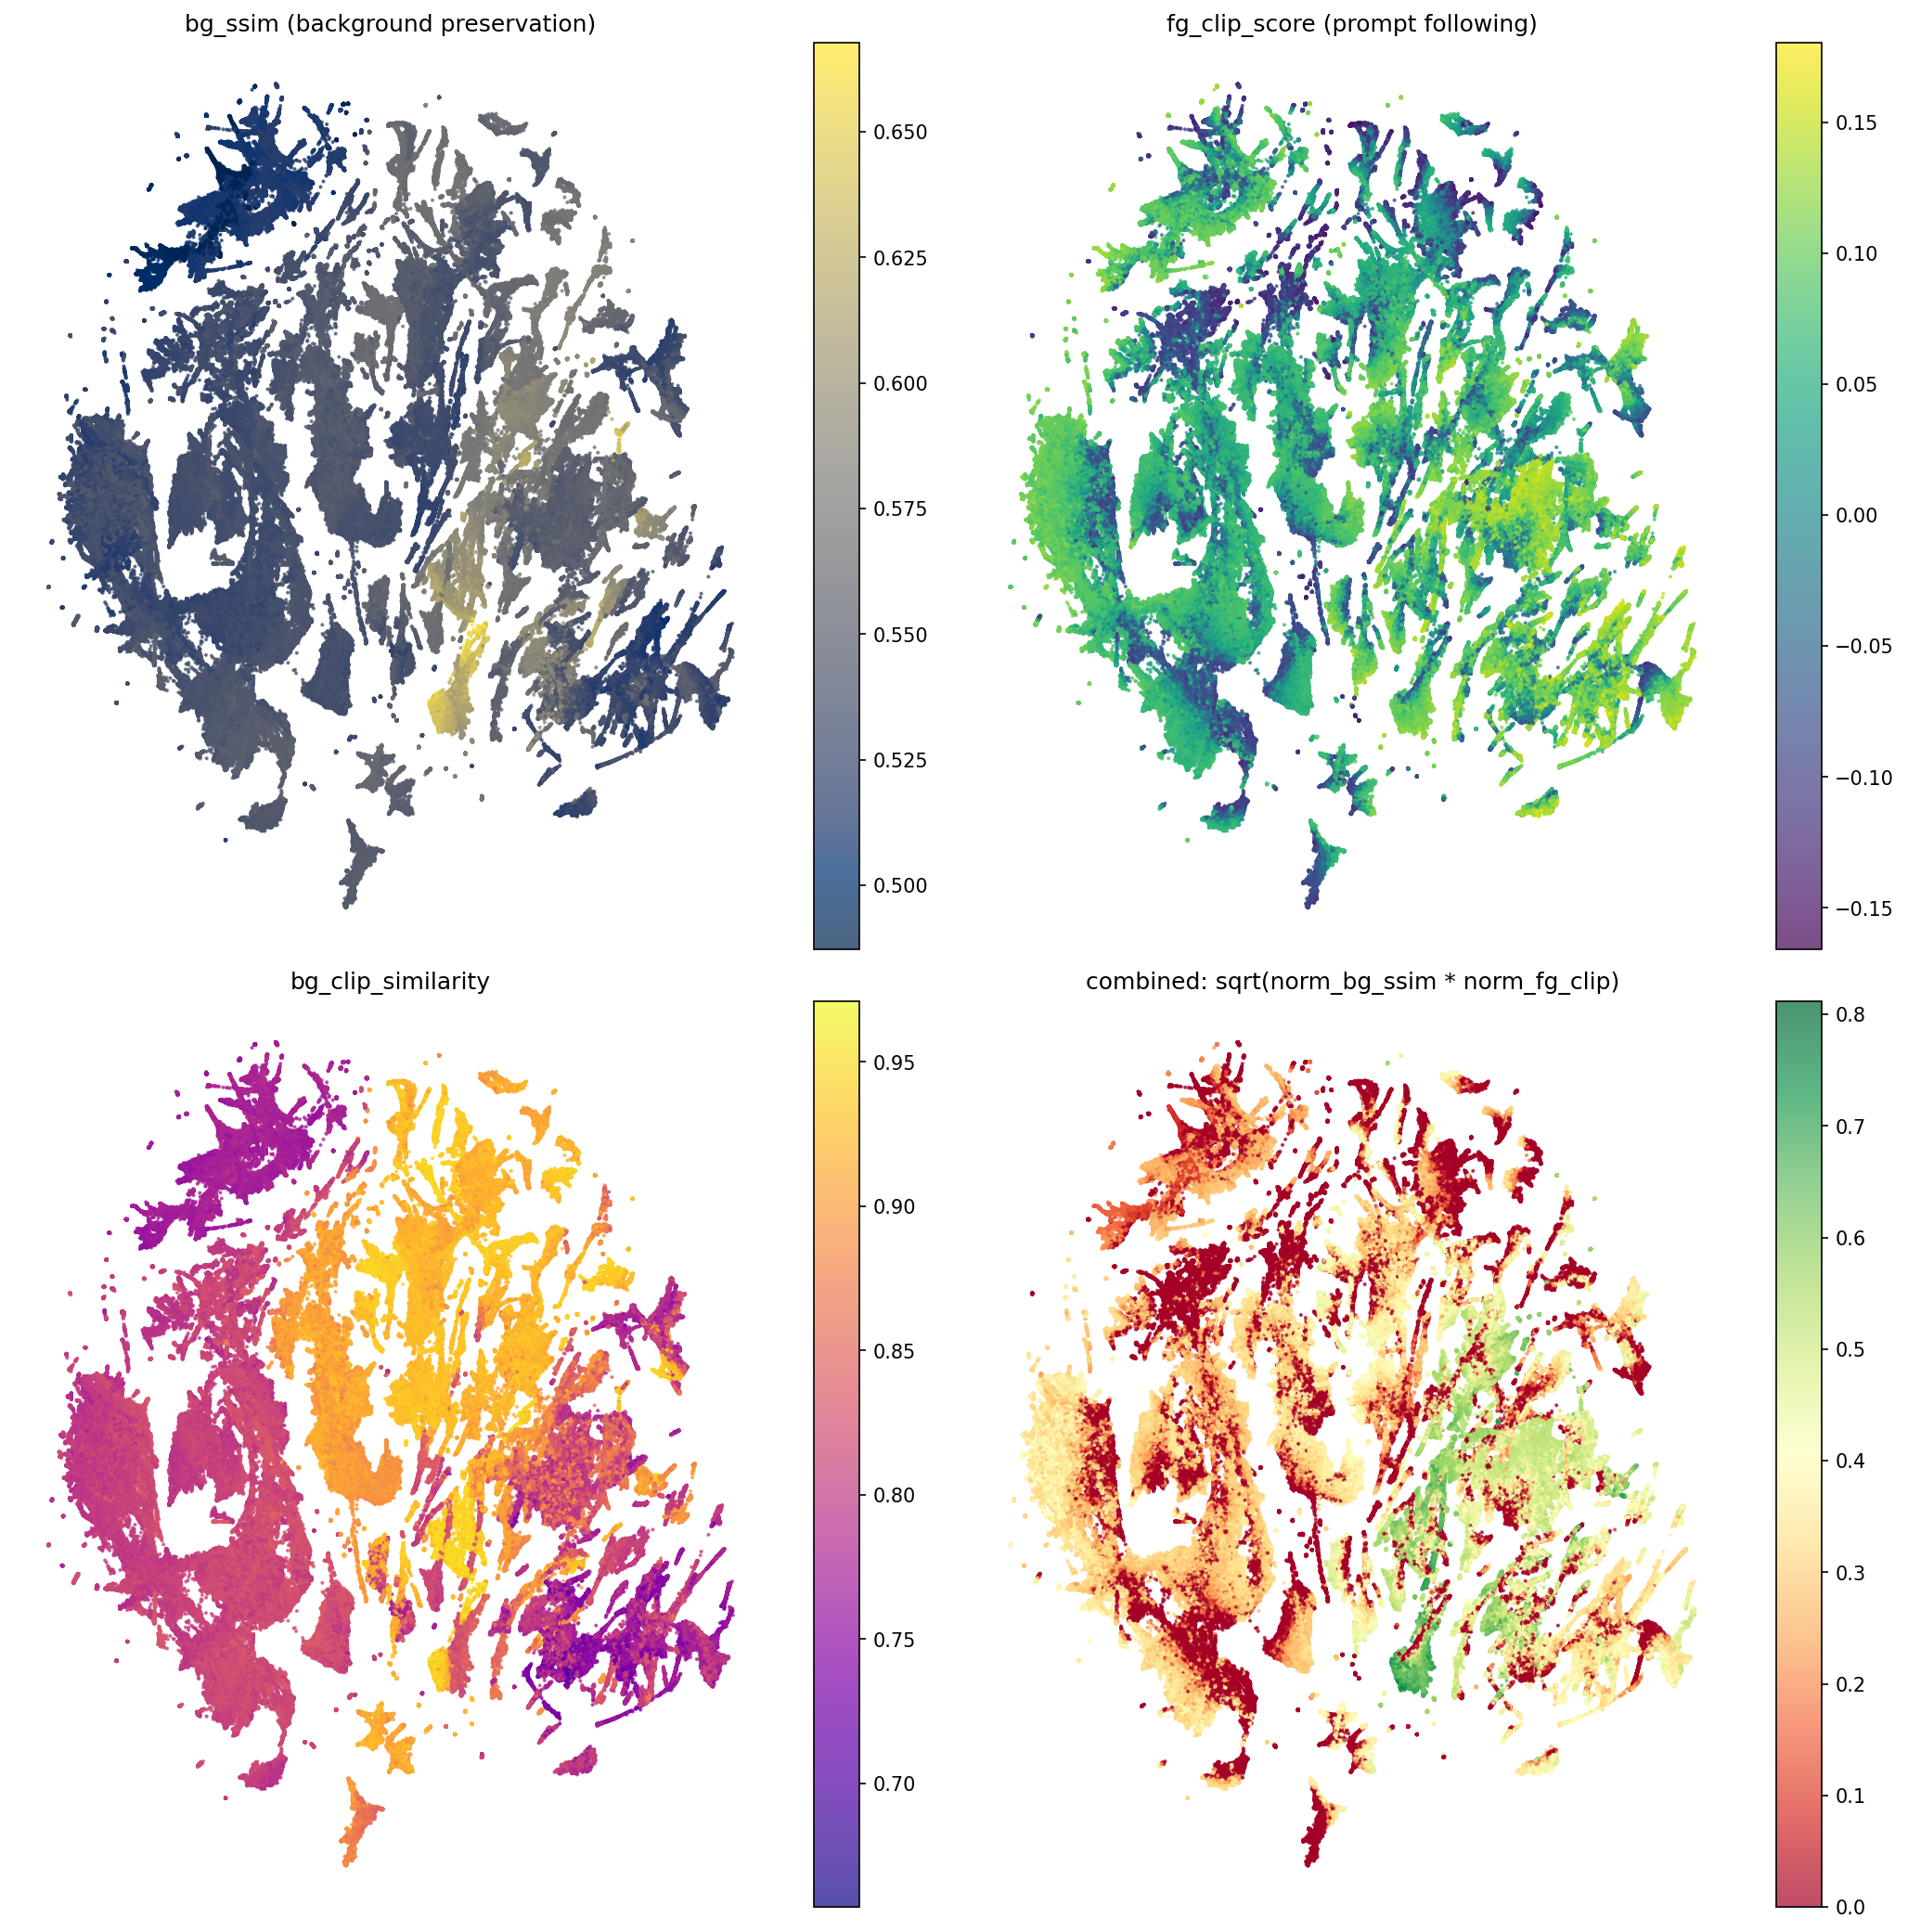
\includegraphics[width=\textwidth]{images/catdog_map_seg_metrics.png}
        \caption{Cat$\to$dog.}
        \label{fig::catdog_metrics}
    \end{subfigure}
    \hspace{0.02\textwidth}
    \begin{subfigure}[t]{0.48\textwidth}
        \centering
        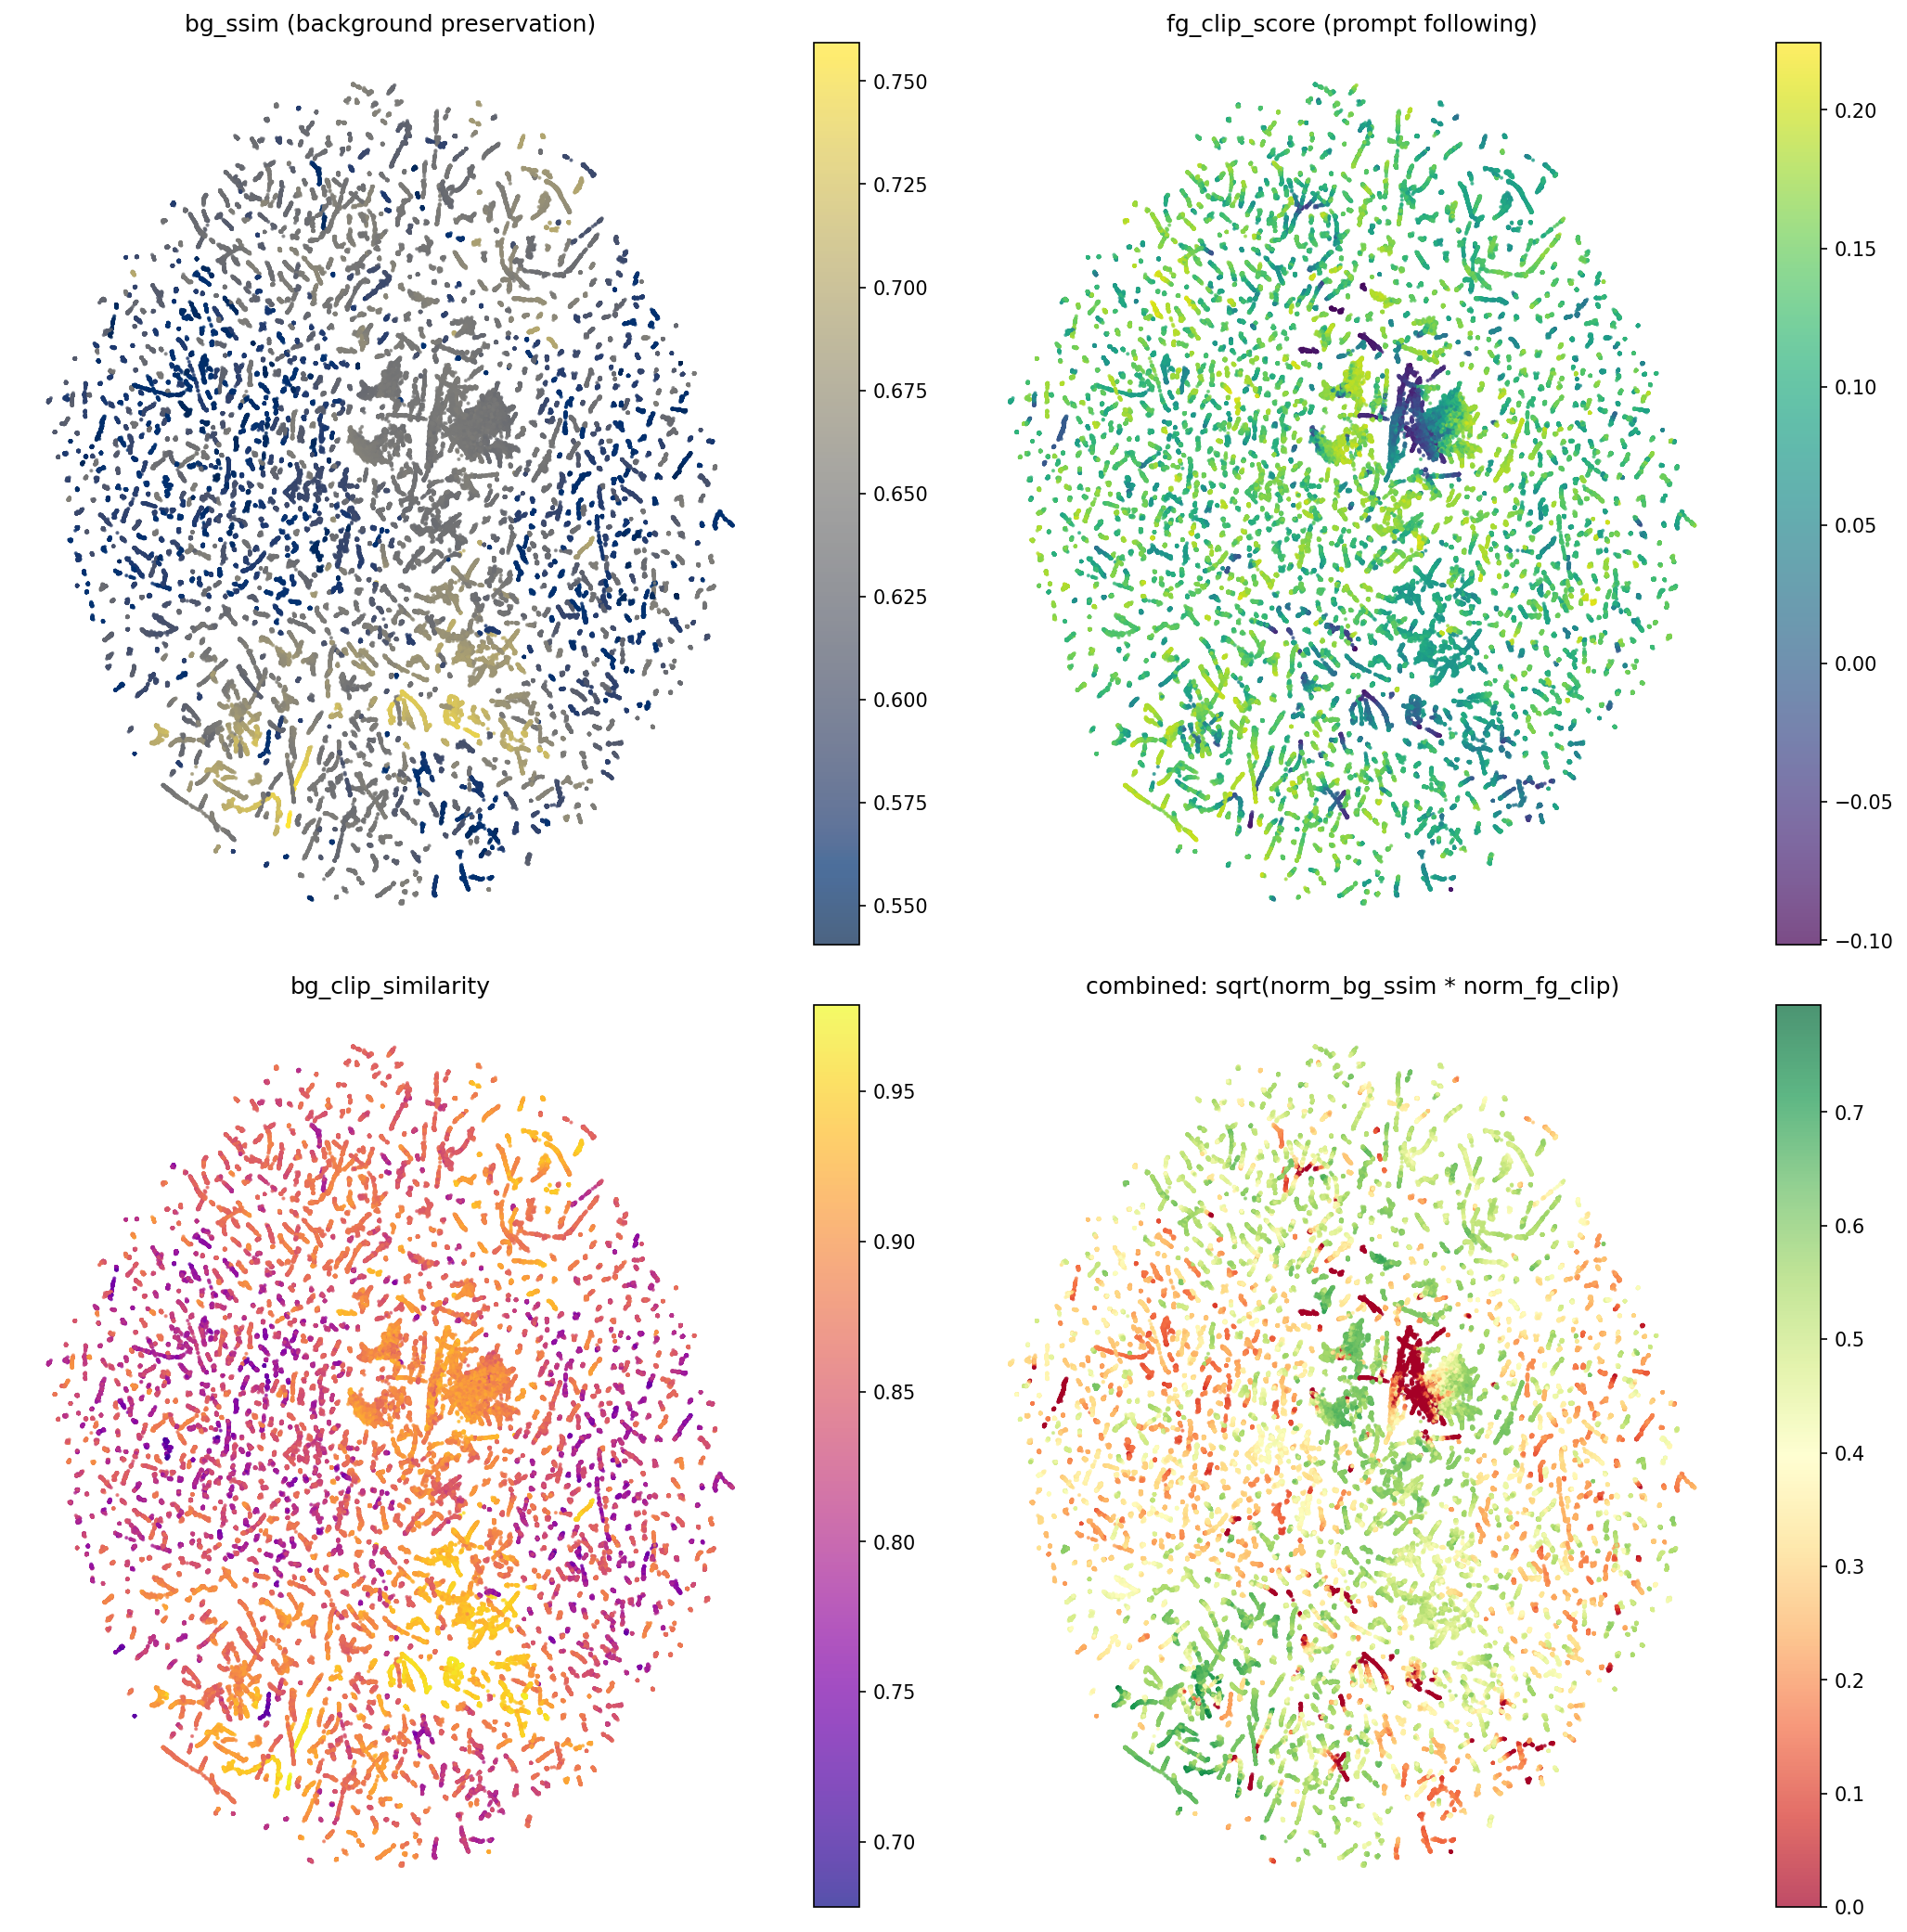
\includegraphics[width=\textwidth]{images/horse_map_seg_metrics.png}
        \caption{Horse$\to$robot horse.}
        \label{fig::horse_metrics}
    \end{subfigure}
    \caption{UMAP projections coloured by metric. Per panel, top-left: $f_{\text{bg-ssim}}$; top-right: $f_{\text{fg-clip}}$; bottom-left: $f_{\text{bg-clip}}$; bottom-right: combined score.}
    \label{fig::metric_maps}
\end{figure}

\section{The all-target mask is not the answer}

Figure~\ref{fig::all_ones_vis} shows side by side, for each task, the source image ($M=\mathbf{0}$, source prompt on every step), the all-target output ($M=\mathbf{1}$, target prompt on every step), and the best mask by combined score ($M^*$, found by exhaustive search). The all-target column destroys part of the scene on both tasks: cat$\to$dog loses the stone-pavement texture and shifts lighting; horse$\to$robot horse bleeds mechanical textures into the grass. The $M^*$ column swaps the object while keeping the scene almost unchanged.

A caveat on artefacts. Stable Diffusion~v1.5 has a documented tendency to produce anatomical and texture glitches (warped limbs, melted hardware, fused objects) on 512$\times$512 outputs; the robot horse in particular shows the ``mechanical-horse'' failure mode that any SD~v1.5 generation of such a prompt will have. These artefacts are a property of the generative backbone, not of the DCS paradigm. The point of Figure~\ref{fig::all_ones_vis} is the background collapse in the $M=\mathbf{1}$ column versus the $M^*$ column, which holds regardless of which backbone generates the foreground.

\begin{figure}[H]
    \centering
    \begin{subfigure}[t]{0.3\textwidth}
        \centering
        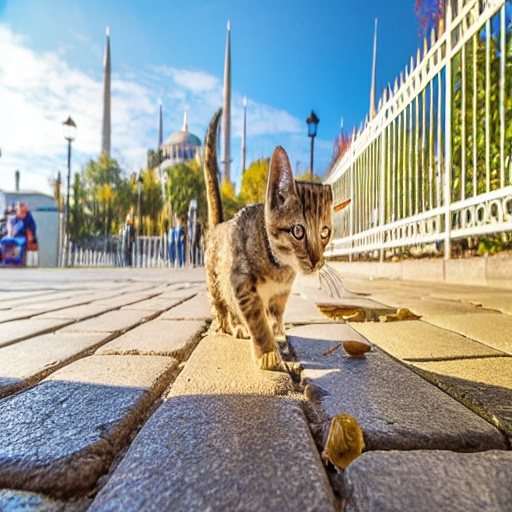
\includegraphics[width=\textwidth]{images/phase1/cat_source.jpg}
        \caption{Cat$\to$Dog: source ($M=\mathbf{0}$)}
    \end{subfigure}
    \hfill
    \begin{subfigure}[t]{0.3\textwidth}
        \centering
        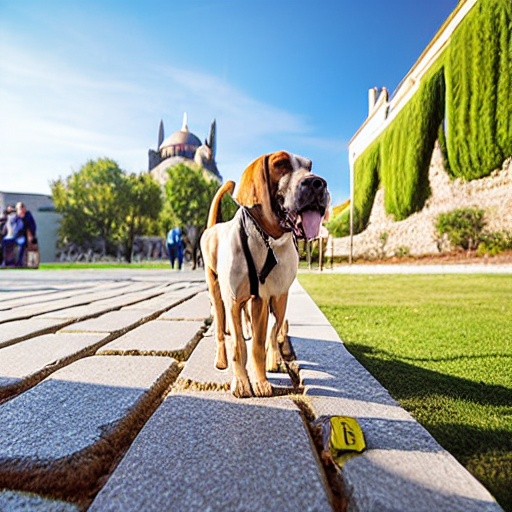
\includegraphics[width=\textwidth]{images/phase1/cat_all_ones.jpg}
        \caption{Cat$\to$Dog: all-target ($M=\mathbf{1}$)}
    \end{subfigure}
    \hfill
    \begin{subfigure}[t]{0.3\textwidth}
        \centering
        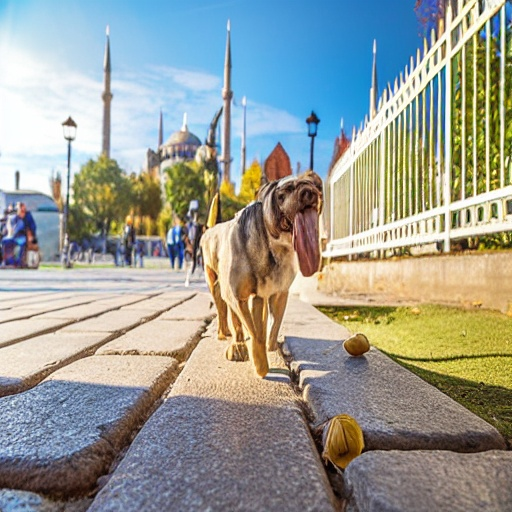
\includegraphics[width=\textwidth]{images/phase1/cat_best.jpg}
        \caption{Cat$\to$Dog: best ($M^*$)}
    \end{subfigure}

    \vspace{0.6em}

    \begin{subfigure}[t]{0.3\textwidth}
        \centering
        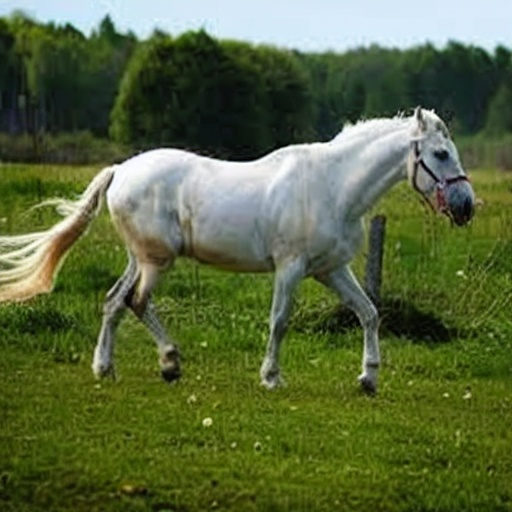
\includegraphics[width=\textwidth]{images/phase1/horse_source.jpg}
        \caption{Horse$\to$Robot horse: source ($M=\mathbf{0}$)}
    \end{subfigure}
    \hfill
    \begin{subfigure}[t]{0.3\textwidth}
        \centering
        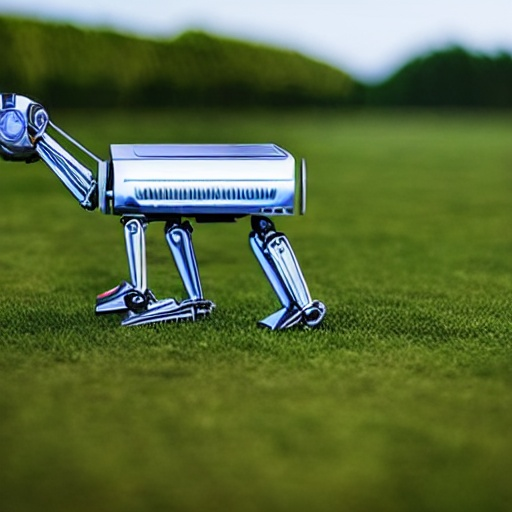
\includegraphics[width=\textwidth]{images/phase1/horse_all_ones.jpg}
        \caption{Horse$\to$Robot horse: all-target ($M=\mathbf{1}$)}
    \end{subfigure}
    \hfill
    \begin{subfigure}[t]{0.3\textwidth}
        \centering
        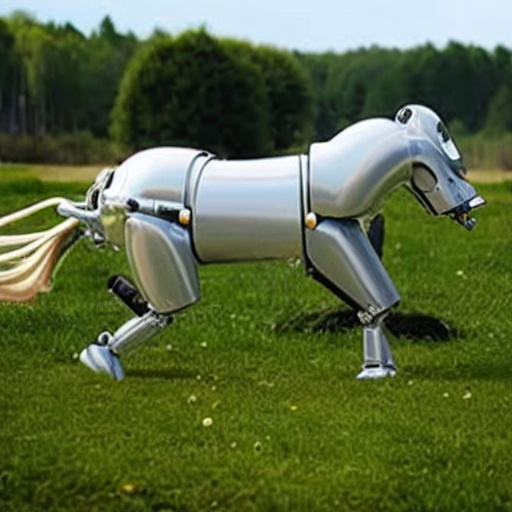
\includegraphics[width=\textwidth]{images/phase1/horse_best.jpg}
        \caption{Horse$\to$Robot horse: best ($M^*$)}
    \end{subfigure}
    \caption{Three masks per task: source $M=\mathbf{0}$ runs the source prompt on every step, all-target $M=\mathbf{1}$ runs the target prompt on every step, $M^*$ is the top-combined mask from the $2^{20}$ exhaustive search. The $M=\mathbf{1}$ column breaks the background on both tasks; $M^*$ keeps it. Foreground artefacts (blurred anatomy, melted mechanical parts) are an SD~v1.5 backbone limitation, not a DCS property.}
    \label{fig::all_ones_vis}
\end{figure}

Figure~\ref{fig::top_combined_grids} shows the 20 masks with the highest combined score on each task. Winning masks activate few target bits in Q1 ($q_1\in[0,2]$), a moderate number in Q2 and Q3 ($q_2, q_3\in[1,3]$), and a variable number in Q4. Source conditioning dominates the early, high-noise timesteps; target conditioning takes over later. Both tasks show the same pattern.

\begin{figure}[H]
    \centering
    \begin{subfigure}[t]{0.48\textwidth}
        \centering
        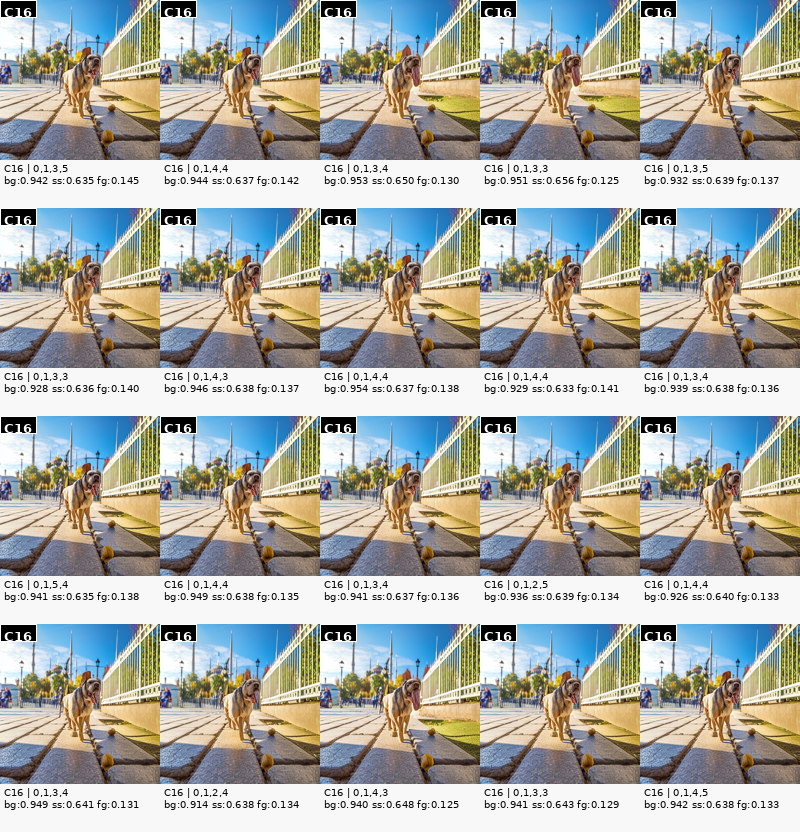
\includegraphics[width=\textwidth]{images/catdog_grid_top_combined.png}
        \caption{Cat$\to$dog.}
        \label{fig::catdog_top_combined}
    \end{subfigure}
    \hspace{0.02\textwidth}
    \begin{subfigure}[t]{0.48\textwidth}
        \centering
        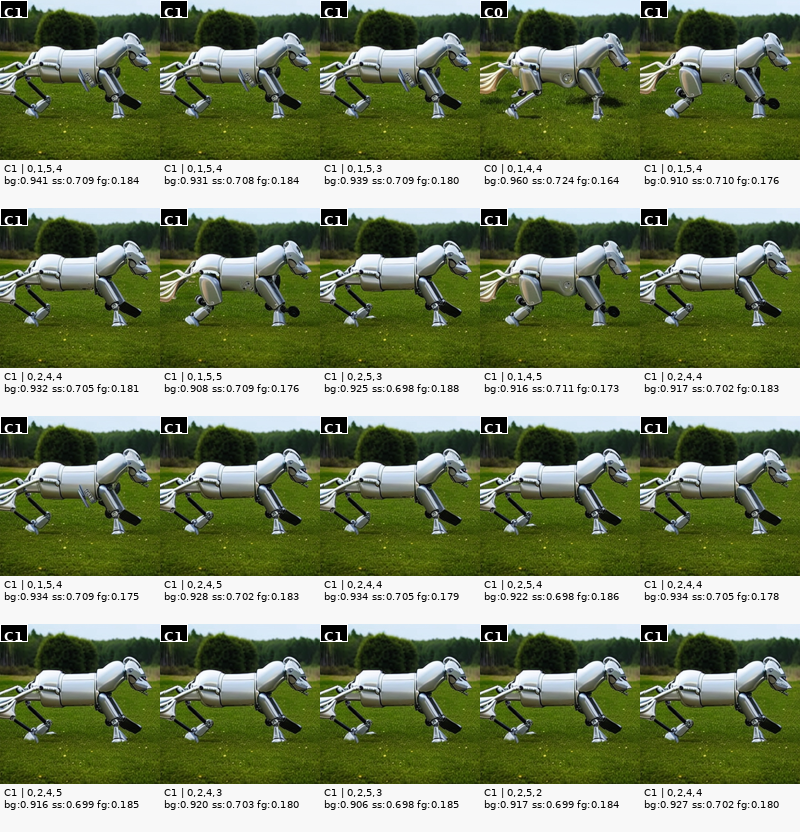
\includegraphics[width=\textwidth]{images/horse_grid_top_combined.png}
        \caption{Horse$\to$robot horse.}
        \label{fig::horse_top_combined}
    \end{subfigure}
    \caption{Top-20 masks by combined score per task. Annotations per image show mask bits (MSB-first) and raw metric values.}
    \label{fig::top_combined_grids}
\end{figure}

\section{Takeaway}

\begin{table}[H]
    \centering
    \caption{Exhaustive-search summary (SD~v1.5, $2^{20}$ masks per task).}
    \begin{tabular}{lcc}
    \toprule
    & \textbf{Cat $\to$ Dog} & \textbf{Horse $\to$ Robot} \\
    \midrule
    Trajectories & 1{,}048{,}576 & 1{,}048{,}576 \\
    HDBSCAN clusters & 52 & 13 \\
    All-ones combined score & 0.220 & 0.167 \\
    Best combined score & 0.885 & 0.826 \\
    \% masks above all-ones & 95.7\% & 98.1\% \\
    Optimal pattern & Source-early, target-late & Source-early, target-late \\
    \bottomrule
    \end{tabular}
    \label{tab::summary}
\end{table}

The $2^{B}$ binary trajectory space splits into dozens of visually distinct clusters. The per-task optimum lives in a source-early / target-late sub-region that the all-target mask does not reach; on both tasks, more than $95\%$ of random masks beat it. A practical editing method therefore needs a search procedure that finds these non-trivial masks without enumerating all $2^{B}$ of them. The next chapter builds that procedure: REINFORCE on 14 Bernoulli logits, running on the FLUX.2 backbone.
